\documentclass[12pt]{article}

\usepackage[utf8]{inputenc}
\usepackage{geometry}
\geometry{a4paper,scale=0.75}
\linespread{1.5}
\usepackage{graphicx} 
\usepackage{float} 
\usepackage{subcaption} 
\usepackage{enumerate}
\usepackage{enumitem}
\usepackage{amsmath}
\usepackage{array}
\usepackage{booktabs}
\usepackage{multirow}
\usepackage{amsfonts}
\usepackage[english]{babel}
\usepackage{amsthm}
\usepackage{dcolumn}
\usepackage{multicol}
\usepackage{stfloats}
\usepackage{lscape}
\usepackage[figuresright]{rotating}
\RequirePackage{pdflscape}
\usepackage[toc,page]{appendix}
\usepackage{geometry}
\usepackage{longtable}
\usepackage{comment}
\usepackage{xcolor}

% -------- enumerated sub-labels (a), (b), … --
\usepackage{enumitem}
\setlist[enumerate,1]{label=(\alph*),ref=\alph*}
% ---------------------------------------------

\usepackage{hyperref}
\hypersetup{hidelinks,
	colorlinks=true,
	allcolors=black,
	pdfstartview=Fit,
	breaklinks=true}
\usepackage{csquotes}
\usepackage{natbib}
\bibliographystyle{apalike}
\newtheorem{definition}{Definition}
\newtheorem{theorem}{Theorem}
\newtheorem{proposition}[theorem]{Proposition}
\newtheorem{lemma}[theorem]{Lemma}
\newtheorem{corollary}[theorem]{Corollary}
\newtheorem*{remark}{Remark}
\newtheorem{example}{Example}
\newtheorem{exercise}{Exercise}
\newtheorem{assumption}{Assumption}[section] % number within sections


\begin{document}

\begin{center}
    ECON 4999B: Quantitative Macroeconomics with AI Integration\\
    {\large \textbf{Tutorial Note: Univariate Time Series Analysis}}\\
    Teaching Assistant: Harlly Zhou
\end{center}

The main reference for this tutorial is \textit{Econometrics} by Fumio Hayashi and \textit{Time Series: Theory and Methods} by Peter J. Brockwell and richard A. Davis.

\section{Basic Properties: Stationarity and Ergodicity}
A \textbf{univariate time series data} $\mathbf{X}$ is a sequence of random variables $\{x_t\}$ ordered by time. It is a random variable at each period $t$. Therefore, we can consider several statistics on the $x_t$:
\begin{itemize}
    \item Mean: $\mathbb{E}x_t = \mu_t$;
    \item Variance: $\gamma_t(0) = \operatorname{Var}(x_t) = \mathbb{E}(x_t - \mu_t)^2$;
    \item Autocovariance: $\gamma_t(k) = \operatorname{Cov}(x_t, x_{t-k}) = \mathbb{E} [(x_t - \mu_t)(x_{t-k} - \mu_{t-k})]$;
    \item Autocorrelation: $\rho_t(k) = \frac{\gamma_t(k)}{\sqrt{\gamma_t(0)} \sqrt{\gamma_{t-k}(0)}}$.
\end{itemize}

However, if the distribution of each period is totally different, the study of time series data will be of great difficulty. Therefore, we need several good properties so that the study is more tractable. The first of them is \textbf{stationarity}. It has two different notions, \textbf{strong stationarity} and \textbf{weak stationarity}.

\begin{definition}[strong stationarity]
    A time series $\{x_t\}$ is \emph{strongly stationary} if given $k$, the joint distribution of $(x_t, \cdots, x_{t-k})$ is the same for all $t$. 
\end{definition}
This is a very strict condition. We can consider a weaker version, which is already enough for many scenarios.

\begin{definition}[weak stationarity]
    A time series $\{x_t\}$ is \emph{weakly stationary} if its first (mean) and second moments (variance, autocovariances) are time invariant and finite.
\end{definition}
Using the notation, we require that
\begin{itemize}
    \item Mean: $\mathbb{E}x_t = \mu < \infty$;
    \item Variance: $operatorname{Var}(x_t) = \gamma(0) < \infty$;
    \item Autocovariance: $\operatorname{Cov}(x_t, x_{t-k}) = \gamma(k) < \infty $.
\end{itemize}
Regarding the second moments, weak stationarity says that the variance and autocovariances only differ when the distance between the two periods but do not depend on which period the observation is exactly is.

The second good property is called \text{ergodicity}. We can only observe a part of a time series data as a sample. However, we have no idea what the population looks like. Whether the \textit{Law of Large Numbers} and \textit{Central Limit Theorem} still hold in the time series, that is, whether sample moments can be used to make inference on population moments, will depend on the notion of ergodicity.
\begin{definition}[ergodicity]
    A (weakly) stationary process is \emph{ergodic} if, for any measurable function $g(\cdot)$ with $\mathbb{E} |g(X_t)| < \infty$,
    \begin{align*}
        \frac{1}{T} \sum_{t=0}^T g(X_t) \xrightarrow{p} \mathbb{E}[g(X)].
    \end{align*}
\end{definition}
You do not need to worry too much about $\xrightarrow{p}$, which means ``convergence in probability''. Since we care about important moments, we can analogously define what ergodicity in mean and ergodicity in variance mean by taking $g(X_t) = X_t$ and $g(X_t) = (X_t - \mu)^2$, respectively.

It is worth mentioning that there is another statistic called \textbf{long-run variance} for the time series data. It is defined as follows:
\begin{align*}
    LRV(X_t) = \sum_{k=-\infty}^{+\infty} \gamma(k) = \gamma(0) + 2\sum_{k=1}^{+\infty} \gamma(k).
\end{align*}
Note that this is very different from the population variance as this definition also adds up the covariances. Therefore, you cannot use the convergence result from ergodicity. In the identification problems regarding time series, the variances used will usually be this long-run variance. It can be estimated using a method called \textit{Newey-West method}. Please learn the basics of the method by yoursefl. You can specify this method in the footnote of related tables and figures in your writing. 

\section{Representation of Time Series}
With the notion of stationarity in hand, we are ready to analyze the time series. It is understandable that a time series will have some deterministic parts which can be predicted and some random parts which are considered as ``shocks''. Is this decomposition generally true in theory? The answer is yes, under some conditions:
\begin{theorem}(Wold decomposition)
    Any zero-mean weakly stationary time series $\{x_t\}$ can be decomposed as $x_t = d_t + y_t$ where $y_t = \sum_{i=0}^{+\infty} \psi_i e_{t-i}$ such that
    \begin{itemize}
        \item $\psi_0 = 1$, $\sum_{i=0}^{+\infty} \psi_i^2 < \infty$;
        \item $e_t := x_t - \mathcal{P}(x_t | x_{t-1}, x_{t-2}, \cdots) \sim WN(o, \sigma^2)$, a \textbf{white noise} process with $\sigma > 0$, that is, $\mathbb{E} e_t = 0$, $\mathbb{E} [e_t e_s] = 0, \forall t\neq s$, and $\operatorname{Var}(e_t) = \sigma^2$;
        \item $\mathbb{E}[e_t d_s] = 0, \forall t, s$; and
        \item $d_t = \mathcal{P}(d_t | x_{t-1}, x_{t-2}, \cdots)$.
    \end{itemize}
\end{theorem}
Here the notation $\mathcal{P}(X|Y)$ means that projection of $X$ onto $Y$. Using words, $\mathcal{P}(X|Y)$ represents the components in $X$ that can be explained/predicted by $Y$. Therefore, the definition of $e_t$ says that $e_t$ is the unpredictable parts of the time series $x_t$, and the definition of $d_t$ says $d_t$ is just the part of itself that can be explained by the history, that is, the whole part is predictable (deterministic).

The Wold decomposition theorem is useful in the sense that now we may write a stationary time series as a sum of its histories and shocks. This kind of representation is called a \textbf{Autoregressive Moving Average $(p,q)$} ($ARMA(p,q)$) representation:
\begin{align*}
    x_t = c + \alpha_1 x_{t-1} + \alpha_2 x_{t-2} + \cdots + \alpha_p x_{t-p} + e_t + \theta_1 e_{t-1} + \theta_2 e_{t-2} + \cdots + \theta_q e_{t-q},
\end{align*}
where $c$ is a constant and $e_s$ are white noise for all $s$. The part with histories and the current noise $e_t$ is the $AR$ part, and that with only shocks is the $MA$ part. 

This representation is not compact. To make the expression compact, we introduce the \textbf{lag operator} $L$. It works in the way such that $L x_t = x_{t-1}$ and $L^p x_t = x_{t-p}$. Using this operator, we can write the $ARMA(p,q)$ expression introduce
\begin{align*}
    (1 - \alpha_1 L - \alpha_2 L^2 - \cdots - \alpha_p L^p) x_t = c + (1 + \theta_1 L + \theta_2 L^2 + \cdots + \theta_q L^q) e_t,
\end{align*}
This is still not compact enough since there is the sum of many items. We can use the notation of a \textbf{filter} to make the expression more compact:
\begin{align*}
    \alpha(L) x_t = c + \theta(L) e_t,
\end{align*}
where $\alpha(L) = 1 - \alpha_1 L - \alpha_2 L^2 - \cdots - \alpha_p L^p$, and $\theta(L) = 1 + \theta_1 L + \theta_2 L^2 + \cdots + \theta_q L^q$. A filter can in general be written as $G(L) = g_0 + g_1 L + g_2 L^2 + \cdots$. Note that a property of filter is that when you apply a filter onto a constant (time-invariant), you are essentially applying the lag operator on a constant time series, \textit{i.e.}, $c_t = c$ for all $t$. In this case, we can write $G(1)$ as applied to the time series such that $G(1) = g_0 + g_1 + g_2 + \cdots$. Under this convention, we have
\begin{align*}
    x_t = \mu + \psi(L) e_t
\end{align*}
where $\mu = \frac{c}{\alpha(1)}$ and $\psi(L) = \frac{\theta(L)}{\alpha(L)}$. It is clear that $\mathbb{E} x_t = \mu$ since $\{x_t\}$ is staionary and $e_t \sim WN(0, \sigma^2)$.

\subsection{Moving Average Representation}
We first try to understand the $MA(q)$ representation. Suppose a stationary time series $\{x_t\}$ can be represented by the following expression:
\begin{align*}
    x_t &= \mu + e_t + \theta_1 e_{t-1} + \theta_2 e_{t-2} + \cdots + \theta_q e_{t-q}\\
    &= \mu + \theta(L) e_t.
\end{align*}
Think about the economics of this expression: a new realization of the a time series is its mean and the accumulation of past shocks. An example will be something like the efficient market hypothesis: the stock prices will reflect the arrival of \textit{unexpected} news. But in research, whether a component is predictable or unpredictable is not directly observed in data. Therefore, this $MA(q)$ expression provides with us a good way to back out the ``shock'' component $e_t$ in the current period using the observed $x_t$ and its mean. At a first glance, this is easy in the sense that we can just take $\theta(L)^{-1}$ can we are done. However, this is not true because this filter may not be intrinsically invertible. Before you make this operation, you need to first test the \textbf{invertibility} of the expression.
\begin{proposition}[invertibility condition]
    Consider a stationary time series $\{x_t\}$ with the above $MA(q)$ expression. It is invertible if all the zeros of the following equation lies outside the unit circle of a complex plane $z \in \mathbb{C}$:
    \begin{align*}
        1 + \theta_1 z + \theta_2 z^2 + \cdots + \theta_q z^q = 0.
    \end{align*}
\end{proposition}
Now let's use the following examples to illustrate how this works.
\begin{example}[invertible $MA(2)$]
    Consider the following time series: $x_t = e_t + 0.6 e_{t-1} + 0.08 e_{t-2}$. The characteristic equation is $1 + 0.6 z + 0.08 z^2 = 0$ with two zeros $z_1 = -5$ and $z_2 = -2.5$. Both of them lie outside the unit circle so the time series is invertible. Then we can write
    \begin{align*}
        \frac{1}{(1+0.2L)(1+0.4L)} x_t = e_t.
    \end{align*}
    Using the formula of geometric series, we have
    \begin{align*}
        e_t &= \left(\sum_{i=0}^{+\infty}(-0.2)^i L^i\right)\left(\sum_{i=0}^{+\infty}(-0.4)^i L^i\right) x_t \\
        &= \left[\left(\sum_{i=0}^{+\infty}(-0.4)^i L^i\right) -0.2\left(\sum_{i=0}^{+\infty}(-0.4)^i L^{i+1}\right) + (-0.2)^2\left(\sum_{i=0}^{+\infty}(-0.4)^i L^{i+2}\right) + \cdots \right] x_t\\
        &= (1 - 0.6L + 0.28 L ^2 + \cdots) x_t.
    \end{align*}
    Now you can find the white noise $e_t$ using the history of $\{x_t\}$.
\end{example}
Let's see one example of non-invertibility.
\begin{example}[invertibility fails]
    Consider the following time series: $x_t = e_t + 2 e_{t-1}$. The root is obviously within the unit circle. If we still use the same way to invert the expression, we have
    \begin{align*}
        e_t = \frac{1}{1+2L} x_t.
    \end{align*}
    However, a geometric series can converge only when the ratio is within the unit circle. Therefore, this $1/(1+2L)$ cannot be expanded as in the previous example. As a result, you cannot back out the $e_t$.
\end{example}

\subsection{Autoregressive Representation}
An $AR$ representation of a time seires is not exclusive to $MA$ representation. They are interchangeable. Consider an $AR(p)$ stationary process, which is the most common representation is the literature for some processes:
\begin{align*}
    x_t = \alpha_1 x_{t-1} + \alpha_2 x_{t-2} + \cdots + \alpha_p x_{t-p} + e_t.
\end{align*}
Our task is now trying to show that we can use an $MA(\infty)$ representation to represent this time series. It is easy to see that
\begin{align*}
    \alpha(L) x_t = e_t.
\end{align*}
This time we are more cautious for this kind of invertibility condition: can $\alpha(L)$ be inverted? Still, we need a similar condition, called the \textbf{stability condition}:
\begin{proposition}[stability condition]
    Consider a stationary time series $\{x_t\}$ with an $MA(p)$ expression. It is stable if all the zeros of the following equation lies outside the unit circle of a complex plane $z \in \mathbb{C}$:
    \begin{align*}
        1 - \alpha_1 z - \alpha_2 z^2 - \cdots - \alpha_p z^p = 0.
    \end{align*}
\end{proposition}

Now we use two examples to explain why this stability condition is economically important:
\begin{example}[$AR(1)$ is $MA(\infty)$]
    Consider a stationary $AR(1)$ process: $x_t = 0.5 x_{t-1} + e_t$. Obviously, it is stable. Then we can write
    \begin{align*}
        x_t &= \frac{1}{1-0.5L} e_t \\
        &= \sum_{i=0}^{+\infty} (0.5)^i L^i e_t\\
        &= e_t + 0.5 e_{t-1} + 0.25 e_{t-2} + \cdots.
    \end{align*}
    We can express an $AR(1)$ process using a $MA(\infty)$ representation.
\end{example}
For $AR(p)$ processes, we can also express them using the $MA(\infty)$ representation. Similar techniques can be used as in Example 1.
\begin{example}[exploding accumulation]
    Consider a stationary $AR(1)$ process: $x_t = 2 x_{t-1} + e_t$. Obviously, it is not stable. So we cannot invert the $\alpha(L)$ filter. However, we can use a backward induction. Note that the expression is true for all $t$'s. So we have
    \begin{align*}
        x_t &= 2(2x_{t-2} + e_{t-1}) + e_t\\
        &= 4(2x_{t-3} + e_{t-2}) + e_t + 2 e_{t-1}\\
        &= 8(2x_{t-4} + e_{t-3}) + e_t + 2 e_{t-1} + 4 e_{t-2}.
    \end{align*}
    Since $e_t$ is a temporary shock for any $t$, its effect should decay with time, so that in a $MA(\infty)$ expression, the coefficients should be less than 1. However, the above backward induction shows that the older the shock is, the larger the effect it has on current variable. This does not make sense.
\end{example}

\section{Empirics of Time Series}
Macroeconomic data are usually in time series. When you bring in some new measurement into your research, it is better to provide some fundamental analysis of the series. A first glance can be its persistence, that is, how does the data fits an $ARMA$ model. Second, how does the variable changes with business cycle? It is cyclical, countercyclical, or acyclical?

\subsection{Estimation of \texorpdfstring{$ARIMA$}{ARIMA} Models}
Recall that in the last section, we mentioned from time to time that all these $ARMA$ representations are only applied to \textit{stationary} time series. However, in practice, many data you get is not stationary. Figure \ref{fig:rgdp-raw} shows the raw US real GDP data. It is clear that the series is not stationary but clearly with an increasing trend. Therefore, we need to first make the series stationary before we can estimate the model, and this is where the letter I in $ARIMA$ comes from. 

\begin{figure}[H]
    \centering
    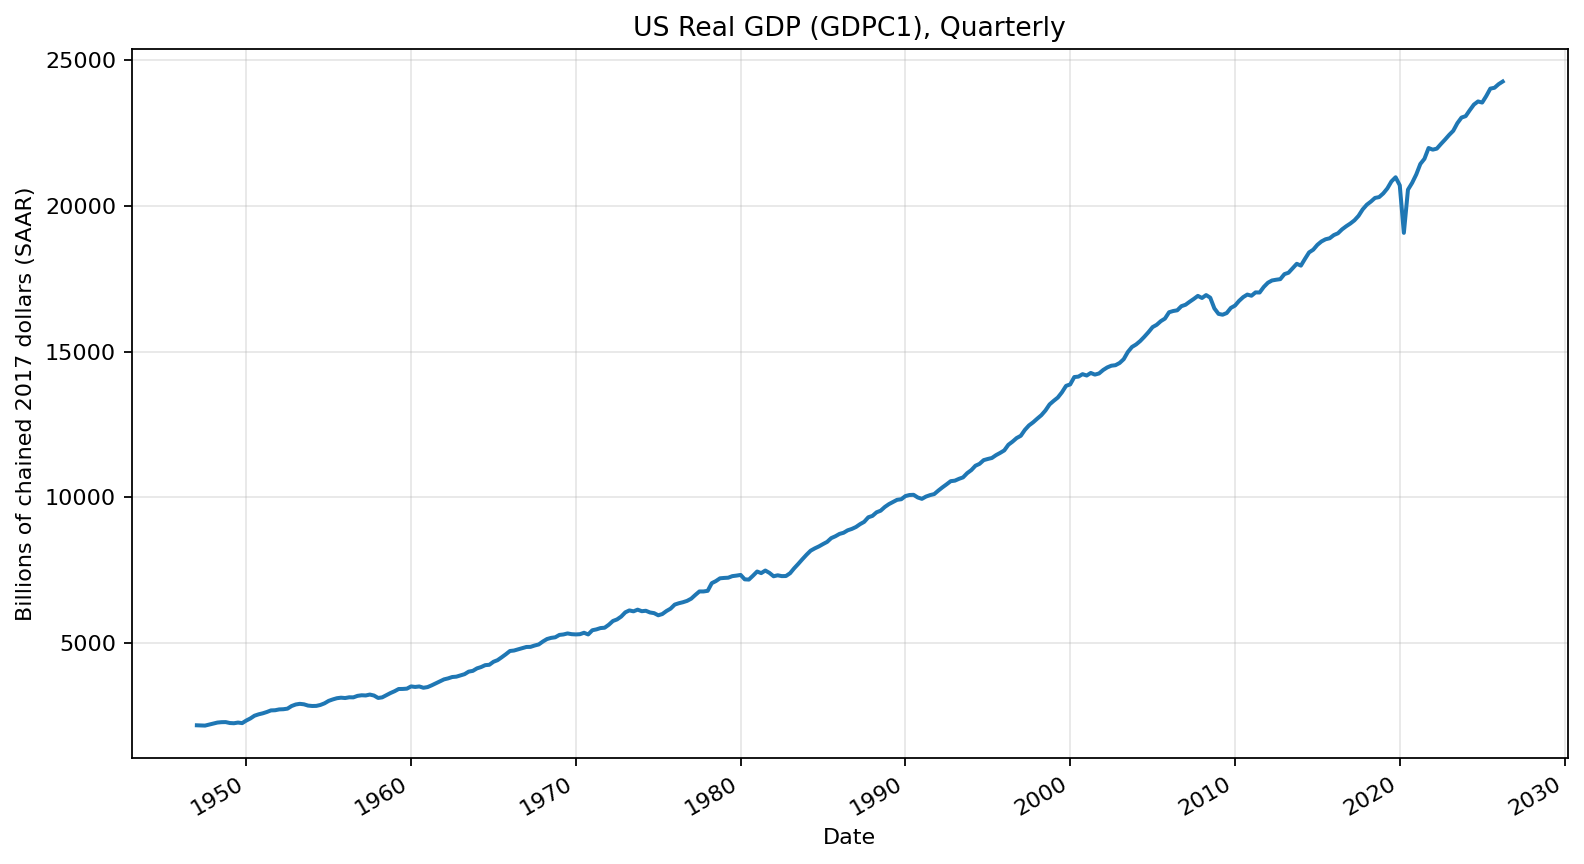
\includegraphics[width=0.6\textwidth]{rgdp_raw.png}
    \caption{US real GDP, quarterly, 1947--2026.}
    \label{fig:rgdp-raw}
\end{figure}

For the GDP series, it is of a large scale. So the first thing we can do is to take logarithm of the series. Then we take a first difference of the series. Note that the log-difference is approximately the percentage change of the series, or in this case, GDP growth rate. From the figure \ref{fig:rgdp-logdiff}, we can see that the series is much more stationary.

\begin{figure}[H]
    \centering
    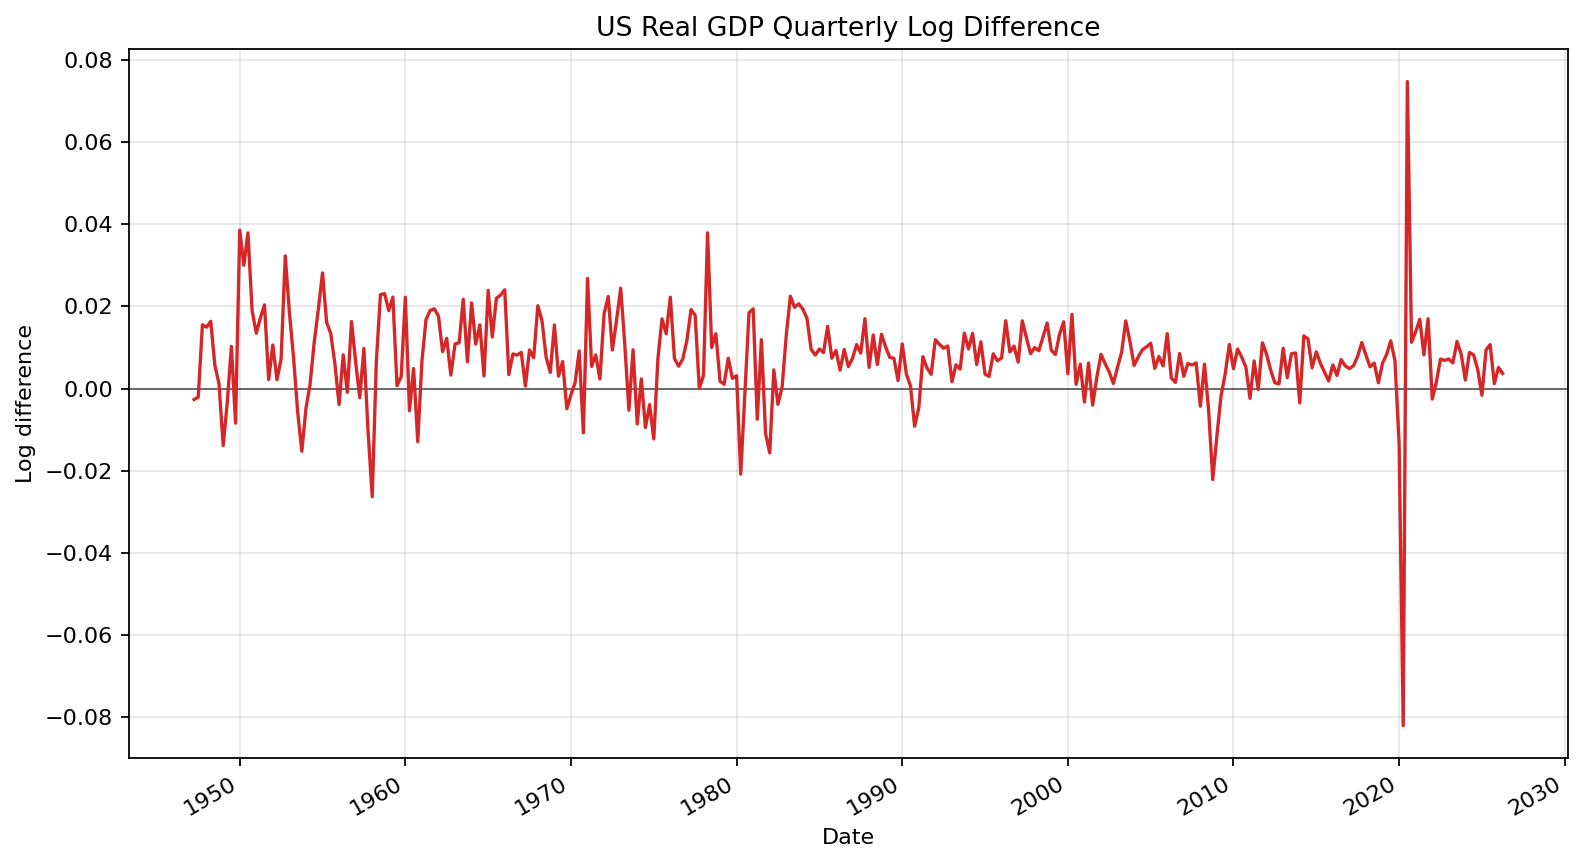
\includegraphics[width=0.6\textwidth]{rgdp_logdiff.png}
    \caption{US real GDP, log difference, quarterly, 1947--2026.}
    \label{fig:rgdp-logdiff}
\end{figure}

However, the mean seems to be significantly different from zero. We can subtract the sample mean from the series to get a zero-mean series so that the Wold decomposition theorem can be applied.

Now we can start to estimate the $ARMA$ model. A handy way is to use the OLS estimation. However, how many lags and lagged shocks should we include, that is, what is the value of $p$ and $q$? There are three ways.

\begin{enumerate}
    \item Box-Jenkins identification using Autocorrelation Function (ACF) and Partial Autocorrelation Function (PACF). The first step of the Box-Jenkins approach is to make the series stationary. Here we have already done so by using the log difference of real GDP. Before applying the Box-Jenkins tools, we subtract the sample mean from the log-difference series so that the analysis focuses on autocovariances. The second step is to use the ACF and PACF of the demeaned stationary series to form candidate values of $p$ and $q$. The ACF is the correlation of the series with its own lags, while the PACF is the correlation after removing the effects of the intermediate lags. In empirical work, we usually plot the sample ACF and PACF together with approximate 95 percent confidence bands. Under the null hypothesis that the stationary series is white noise, the sample autocorrelations are approximately within $\pm 1.96/\sqrt{T}$, where $T$ is the sample size. Bars outside these bands suggest statistically meaningful serial correlation at that lag, while bars inside the bands suggest that the correlation may just be sampling noise. One should not overreact to a single small spike, because when many lags are plotted, one or two spikes can appear by chance.

    The practical Box-Jenkins rule is to look for patterns rather than isolated bars. If the PACF cuts off after lag $p$ and the ACF decays gradually, this suggests an $AR(p)$ model. If the ACF cuts off after lag $q$ and the PACF decays gradually, this suggests an $MA(q)$ model. If both decay gradually, an $ARMA(p,q)$ model may be considered. If both functions are small and mostly within the confidence bands, a parsimonious model with few or no ARMA terms is preferred. In Figure \ref{fig:rgdp-logdiff-acf-pacf}, the ACF are significant at the first two lags while the PACF is significant at the first lag. Therefore, we will pick the $ARMA(1,2)$ model.

    \begin{figure}[H]
        \centering
        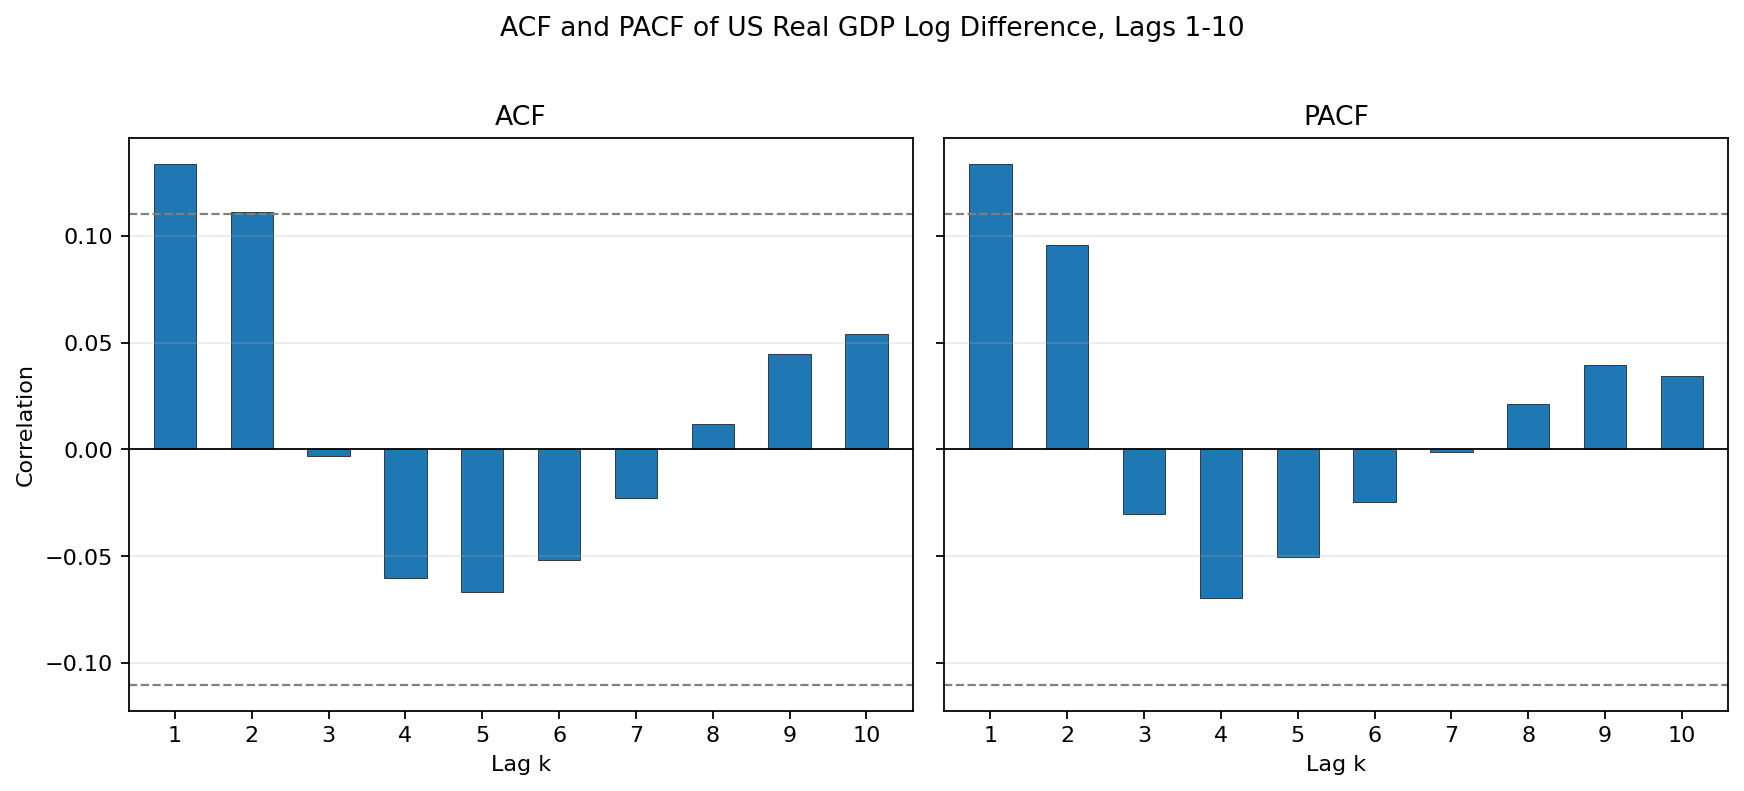
\includegraphics[width=0.85\textwidth]{rgdp_logdiff_acf_pacf.png}
        \caption{ACF and PACF of US real GDP log difference, lags 1--10.}
        \caption*{\footnotesize{Note: The confidence bands are calculated as $\pm 1.96/\sqrt{T}$, where $T$ is the sample size. Shown in dashed lines.}}
        \label{fig:rgdp-logdiff-acf-pacf}
    \end{figure}
    
    \item Akaike Information Criterion (AIC) and Bayesian Information Criterion (BIC). When one compares models, more regressors always increase $R^2$. However, the dimension of the problem will increase exponentially. AIC and BIC are two information criteria that penalize the number of parameters. AIC usually puts a smaller penalty on additional parameters, so it is often useful when the goal is prediction. BIC puts a larger penalty on additional parameters, so it is often preferred when the goal is model selection. When we compare models with different numbers of lags, we should keep the estimation sample fixed. Here, for all lag choices from $p=0$ to $p=10$, we cut the first 10 observations and estimate each $AR(p)$ model on the same remaining sample of demeaned $\Delta \log(\text{GDP})$, without an intercept. With the full GDP sample, AIC selects $p=2$, while BIC still selects the parsimonious $p=0$ model.

    \begin{table}[H]
        \centering
        \caption{AIC and BIC for $AR(p)$ models of demeaned $\Delta \log(\text{GDP})$}
        \label{tab:rgdp-logdiff-aic-bic}
        \begin{tabular}{ccc}
            \toprule
            Lag $p$ & AIC & BIC \\
            \midrule
            0 & -2766.251 & -2766.251 \\
            1 & -2769.018 & -2765.291 \\
            2 & -2770.504 & -2763.050 \\
            3 & -2768.647 & -2757.466 \\
            4 & -2768.074 & -2753.167 \\
            5 & -2766.853 & -2748.219 \\
            6 & -2765.129 & -2742.768 \\
            7 & -2763.165 & -2737.077 \\
            8 & -2761.279 & -2731.464 \\
            9 & -2759.834 & -2726.292 \\
            10 & -2758.274 & -2721.005 \\
            \bottomrule
        \end{tabular}
    \end{table}

    \item Likelihood ratio test. Another way is to compare two nested models directly. For lag choice, we can test the $AR(p)$ model against the restricted $AR(p-1)$ model. The null hypothesis is that the coefficient on the $p$-th lag is zero, so the smaller $AR(p-1)$ model is enough. The likelihood ratio statistic is
    \[
        LR_p = 2\left(\log L_p - \log L_{p-1}\right),
    \]
    which is asymptotically distributed as $\chi^2(1)$ because we add one lag at a time. Using the same demeaned fixed sample as before, the adjacent likelihood ratio tests are reported in Table \ref{tab:rgdp-logdiff-lr}. At the 5 percent level, the test rejects $AR(0)$ against $AR(1)$ but does not reject higher-order additions. At the 10 percent level, the second lag is also marginal. Thus, the LR evidence suggests $p=1$ under a 5 percent threshold and $p=2$ under a 10 percent threshold.

    \begin{table}[H]
        \centering
        \caption{Likelihood ratio tests for adjacent $AR(p)$ models of demeaned $\Delta \log(\text{GDP})$}
        \label{tab:rgdp-logdiff-lr}
        \begin{tabular}{ccc}
            \toprule
            Test & LR statistic & $p$-value \\
            \midrule
            $AR(1)$ vs. $AR(0)$ & 4.767 & 0.029 \\
            $AR(2)$ vs. $AR(1)$ & 3.486 & 0.062 \\
            $AR(3)$ vs. $AR(2)$ & 0.143 & 0.705 \\
            $AR(4)$ vs. $AR(3)$ & 1.428 & 0.232 \\
            $AR(5)$ vs. $AR(4)$ & 0.779 & 0.377 \\
            $AR(6)$ vs. $AR(5)$ & 0.276 & 0.599 \\
            $AR(7)$ vs. $AR(6)$ & 0.036 & 0.851 \\
            $AR(8)$ vs. $AR(7)$ & 0.114 & 0.735 \\
            $AR(9)$ vs. $AR(8)$ & 0.555 & 0.456 \\
            $AR(10)$ vs. $AR(9)$ & 0.440 & 0.507 \\
            \bottomrule
        \end{tabular}
    \end{table}
\end{enumerate}

After picking a candidate $ARIMA(p,d,q)$ model, we can estimate it using OLS, (Generalized) Method of Moment (MoM or GMM), \textbf{Hannan-Rissanen method}, or Maximum Likelihood Estimation (MLE). The Hannan-Rissanen method is useful because it turns the estimation of an $ARMA$ model into a sequence of OLS regressions.

\textbf{Step 1. Estimate a long autoregression.} Choose a relatively large lag length $m$, with $m$ larger than both $p$ and $q$, and estimate
\[
    y_t = c + a_1 y_{t-1} + a_2 y_{t-2} + \cdots + a_m y_{t-m} + u_t
\]
by OLS. Save the residuals from this regression as $\hat e_t$. These residuals are used as proxies for the unobserved shocks.

\textbf{Step 2. Estimate the candidate $ARMA(p,q)$ model.} Run the regression
\[
    y_t
    = c
    + \phi_1 y_{t-1} + \cdots + \phi_p y_{t-p}
    + \theta_1 \hat e_{t-1} + \cdots + \theta_q \hat e_{t-q}
    + v_t
\]
by OLS. The estimated coefficients give $\hat\phi_1,\ldots,\hat\phi_p$ and $\hat\theta_1,\ldots,\hat\theta_q$.

For log real GDP, suppose we estimate an $ARIMA(1,1,2)$ model. Let
\[
    y_t=\Delta\log(\text{GDP}_t).
\]
The Hannan-Rissanen second-stage regression is
\[
    y_t = c + \phi_1 y_{t-1} + \theta_1 \hat e_{t-1} + \theta_2 \hat e_{t-2} + v_t.
\]
Using a first-stage $AR(10)$ model to construct $\hat e_t$, the estimates are reported in the following table.

\begin{table}[H]
    \centering
    \caption{Hannan-Rissanen estimates for $ARIMA(1,1,2)$ of log real GDP}
    \label{tab:rgdp-hr-arima112}
    \begin{tabular}{lccc}
        \toprule
        Parameter & Estimate & Std. Error & $t$-statistic \\
        \midrule
        Constant $c$ & $0.004659^{*}$ & 0.002659 & 1.752 \\
        AR coefficient $\phi_1$ & $0.389570$ & 0.334382 & 1.165 \\
        MA coefficient $\theta_1$ & $-0.268402$ & 0.338886 & -0.792 \\
        MA coefficient $\theta_2$ & $0.077312$ & 0.066730 & 1.159 \\
        \bottomrule
    \end{tabular}
    \caption*{\footnotesize{Note: The dependent variable is $\Delta\log(\text{GDP}_t)$. The second-stage sample has 305 observations. The estimated innovation variance is $1.1504\times 10^{-4}$. $^{***}p<0.01$, $^{**}p<0.05$, $^{*}p<0.10$.}}
\end{table}

For this GDP model, we first test whether the residual mean is zero. The null hypothesis is $H_0:E(v_t)=0$. The result is reported in Table \ref{tab:rgdp-resid-mean-test}.

\begin{table}[H]
    \centering
    \caption{Mean test for residuals from the GDP $ARIMA(1,1,2)$ model}
    \label{tab:rgdp-resid-mean-test}
    \begin{tabular}{cccc}
        \toprule
        Mean of $\hat v_t$ & Std. Error & $t$-statistic & $p$-value \\
        \midrule
        $1.27\times 10^{-18}$ & $6.15\times 10^{-4}$ & 0.000 & 1.000 \\
        \bottomrule
    \end{tabular}
\end{table}

Next, we plot the ACF and PACF of $\hat v_t$. Figure \ref{fig:rgdp-resid-acf-pacf} shows that the residual correlations are well within the confidence bands, so the residuals look close to white noise.

\begin{figure}[H]
    \centering
    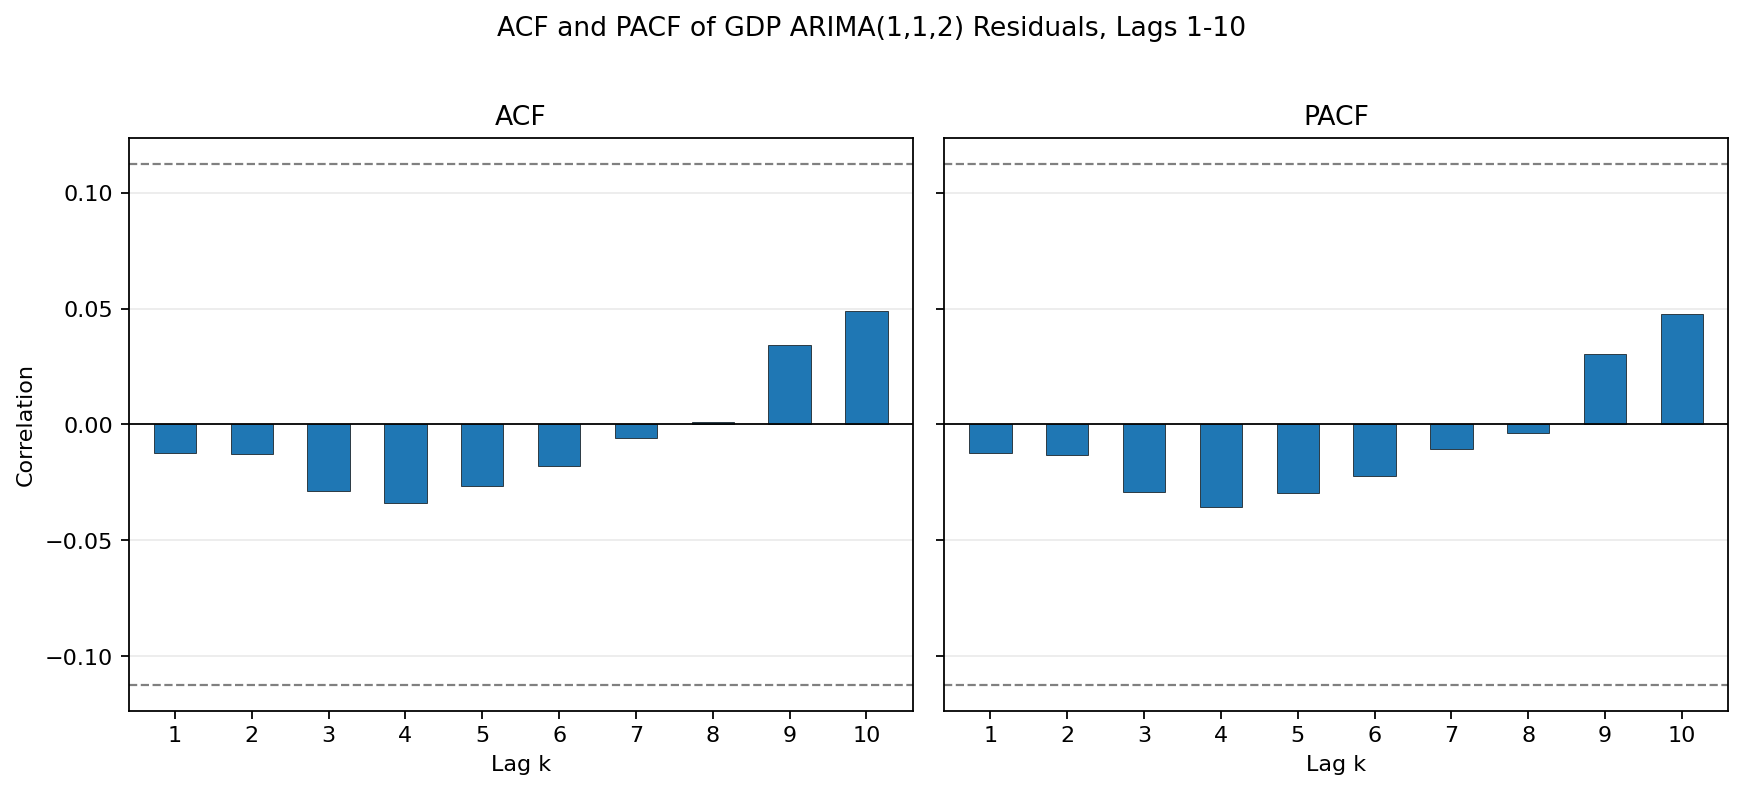
\includegraphics[width=0.8\textwidth]{rgdp_arima112_resid_acf_pacf.png}
    \caption{ACF and PACF of GDP $ARIMA(1,1,2)$ residuals, lags 1--10.}
    \label{fig:rgdp-resid-acf-pacf}
\end{figure}

In general, after estimating an $ARMA$ model, we need to check whether the residual is white noise. We can use the mean, ACF and PACF of the residuals to check this. 

In summary, the complete procedure of estimating an $ARIMA(p,d,q)$ model is as follows:

\begin{center}
\fbox{%
\begin{minipage}{0.95\textwidth}
\textbf{Step 1. Difference the series ($d$).} First, plot the raw series. Try to determine whether the series is stationary or not. If not, take a log difference of the series and plot it as well. Now it seems stationary. Then demean the data so that the Wold decomposition theorem can be applied.

\textbf{Step 2. Estimate the lags ($p, q$).} Use the Box-Jenkins approach to identify the lags. The ACF and PACF of the stationary series are plotted together with the confidence bands. 

\textbf{Step 3. Estimate the model.} Use the Hannan-Rissanen method to estimate the model. The first stage uses a high-order $AR(m)$ model to construct the residuals. The second stage estimates the $ARMA(p,q)$ model using the residuals.

\textbf{Step 4. Check and refine.} Check the residuals of the model. The residuals should be close to white noise. If not, try a different model.
\end{minipage}}
\end{center}

\subsection{Cyclicality in Time Series}
Economists are interested in the business cycle for decades. How are the cycles justified in the data? From the raw data series plotted in the chronological order, there is no clear pattern of cyclicality. However, if we change a perspective -- instead of plotting the series with the $x$-axis as time, we plot the series with the $x$-axis as the angular frequency of the fluctuation, we can see the pattern of cyclicality. The chronological plot is called the \textbf{time domain}, while the frequency plot is called the \textbf{frequency domain}.


Following the real GDP growth rate exercise, we first construct quarterly real GDP growth as $\Delta\log(\text{GDP}_t)$ and subtract its sample mean to focus on autocovariances. In Figure \ref{fig:rgdp-logdiff-frequency}, the top panel shows the demeaned GDP growth rate in the time domain, while the lower four panels show frequency-domain estimates of the population spectrum. The frequency-domain representation is often called the \textbf{spectral representation}. More precisely, these methods estimate the spectrum, or spectral density, of the series. The \textbf{periodogram} is the most direct estimate from the Fourier transform and is plotted as $I(\omega)/(2\pi)$, but it can be noisy. The \textbf{$AR(p)$ spectrum} is parametric and smooth; here $p=2$ is selected by AIC using the full sample. The \textbf{Newey-West kernel estimate} smooths the sample autocovariances using a Bartlett kernel, so it is nonparametric but depends on the bandwidth. Newey-West \textbf{prewhitening} first removes low-order persistence using an $AR(1)$, estimates the spectrum of the residuals, and then recolors the spectrum; this can reduce small-sample bias when the series is persistent.

How do we convert frequency back to periodicity? First, locate the peak angular frequency $\omega$, measured in radians per quarter. Second, compute $T = 2\pi / \omega$. Based on Figure \ref{fig:rgdp-logdiff-frequency}, the periodogram implies a period of about $8.8$ quarters. The $AR(2)$ spectrum peaks essentially at zero frequency, which is best interpreted as a low-frequency component rather than a finite business-cycle periodicity. The Newey-West kernel and prewhitened Newey-West estimates imply periods of about $16.6$ and $22.2$ quarters, respectively. The methods differ because the raw periodogram is noisy, the AR spectrum imposes a parametric shape, and the Newey-West estimators smooth autocovariances nonparametrically. For your knowledge, a typical business cycle periodicity is from 6 quarters to 32 quarters.

\begin{figure}[H]
    \centering
    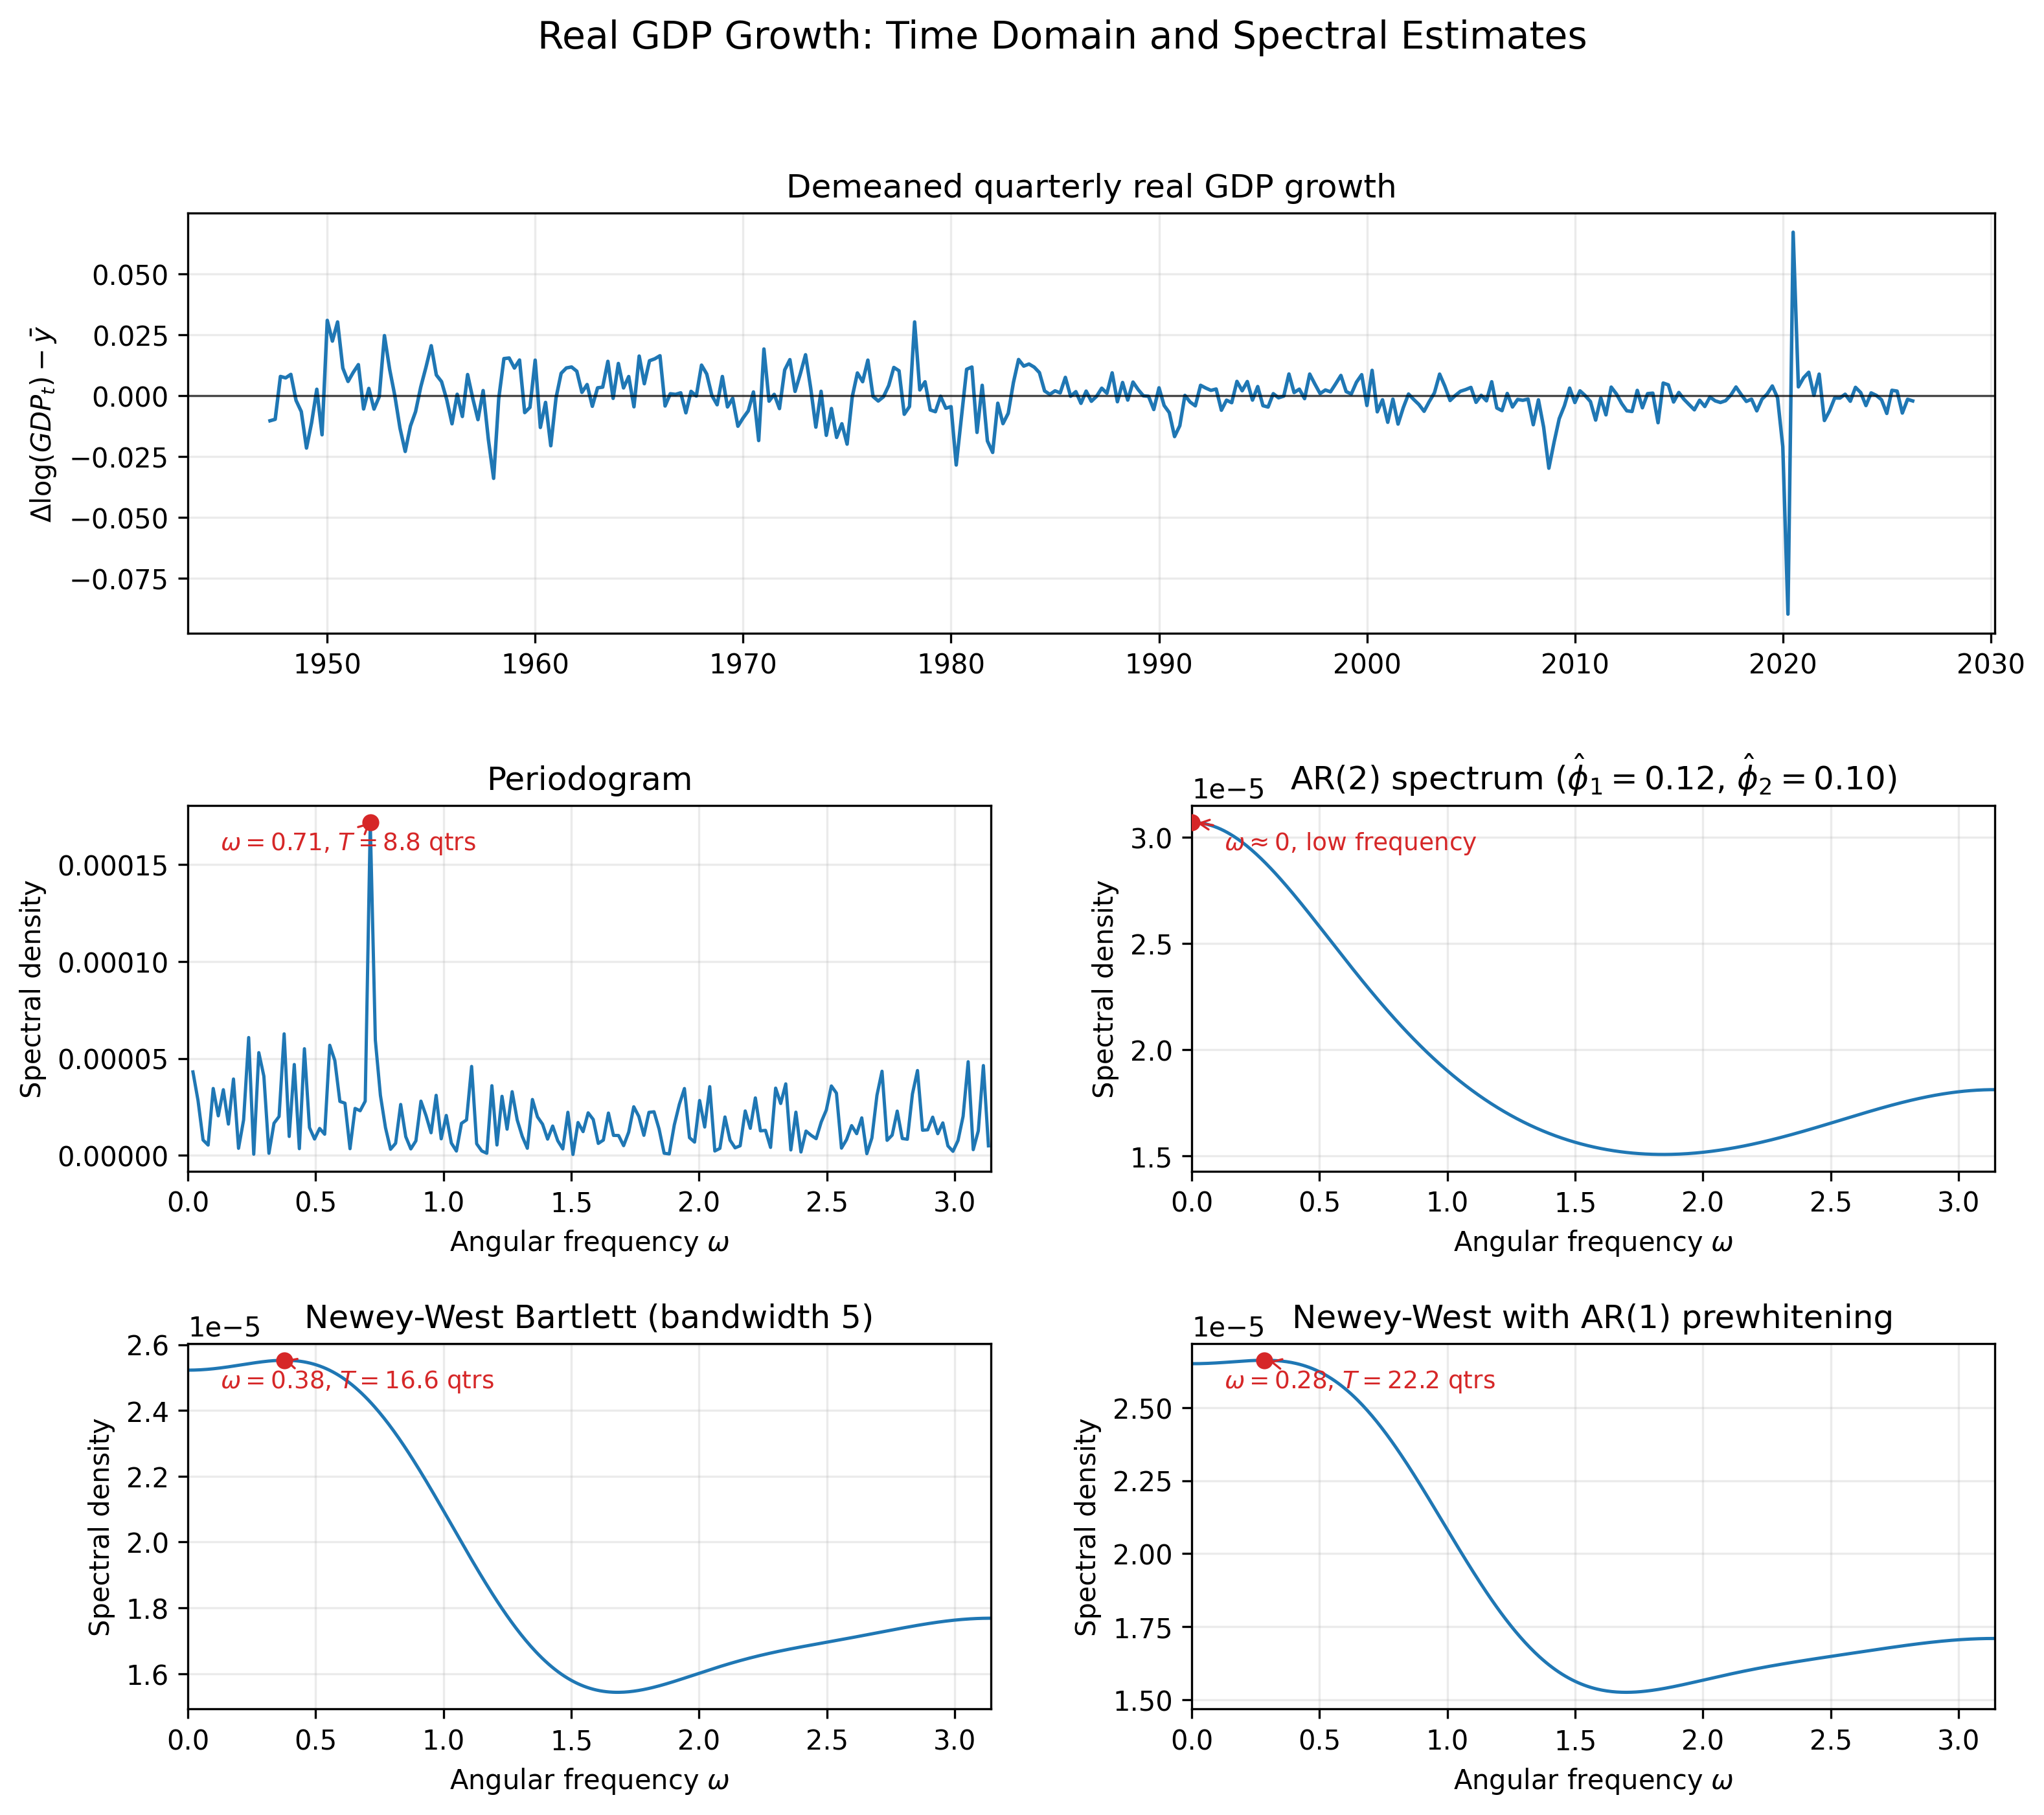
\includegraphics[width=0.9\textwidth]{rgdp_growth_spectrum_hw3_q1.png}
    \caption{US real GDP growth rate in time domain and spectral representations.}
    \label{fig:rgdp-logdiff-frequency}
\end{figure}

Figure \ref{fig:cpi-logdiff-frequency} repeats the same exercise for demeaned CPI log differences, that is, quarterly inflation net of its sample mean. As in the GDP example, the lower four panels report the periodogram, the $AR(p)$ spectrum, the Newey-West kernel estimate, and Newey-West with $AR(1)$ prewhitening. The $AR(p)$ spectrum uses $p=10$, selected by AIC on the full CPI inflation sample. To convert angular frequency into periodicity, use $T=2\pi/\omega$. The periodogram peak is at the lowest positive frequency, $\omega\approx 0.020$, implying $T\approx 316$ quarters. The other spectral estimates also peak essentially at zero frequency, so the dominant movement in CPI inflation is low-frequency inflation persistence rather than a finite business-cycle frequency.

\begin{figure}[H]
    \centering
    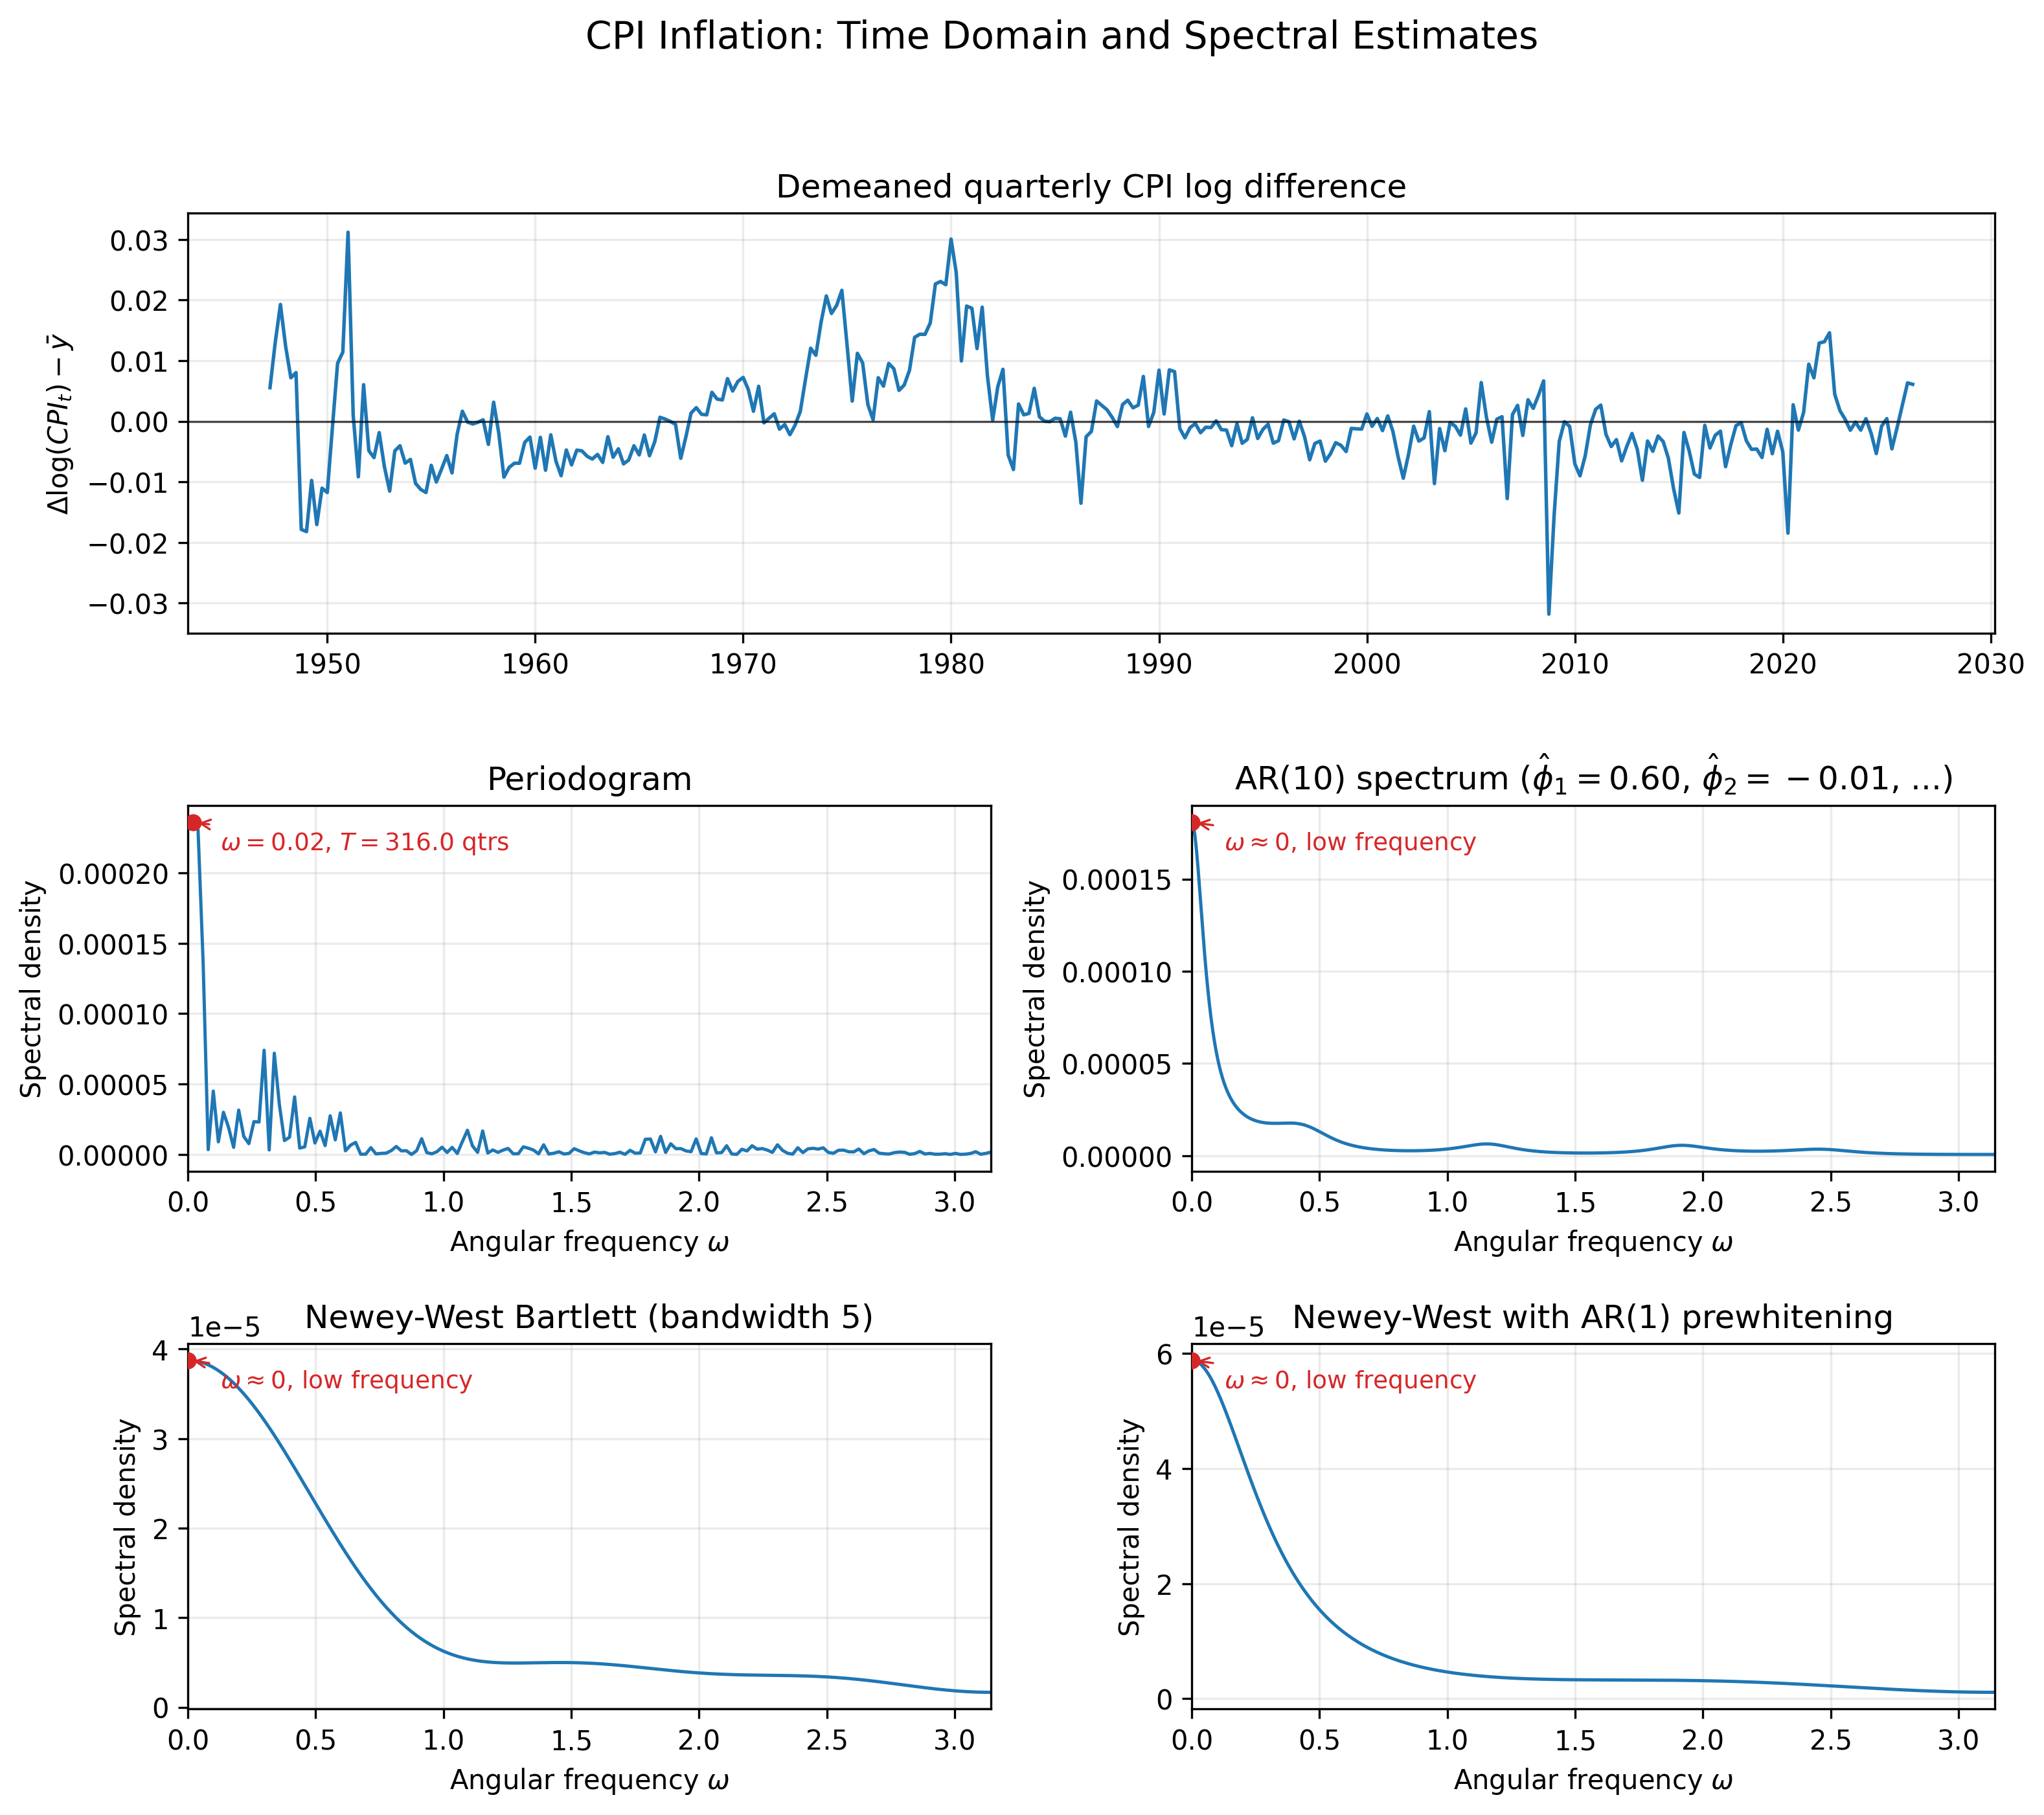
\includegraphics[width=0.9\textwidth]{cpi_logdiff_spectrum_hw3_q1.png}
    \caption{US CPI log difference in time domain and spectral representations.}
    \label{fig:cpi-logdiff-frequency}
\end{figure}

This set of figures seems problematic since the CPI inflation, based on our knowledge, is not persistent. The reason is that we should not plot the raw CPI inflation but the cyclical component. The same should be applied to the GDP growth rate.

How to generate the cyclicality component? We can use the \textbf{Hodrick-Prescott filter (HP filter)}. The HP filter is a smoothing method that decomposes a time series into a trend component and a cyclical component. The trend component is the smoothed series, while the cyclical component is the deviation from the trend. The HP filter is a popular method to generate the cyclicality component because it is simple and easy to implement. Other than the HP filter, the \textbf{band-pass filter} and the \textbf{Christiano-Fitzgerald filter} are also popular methods to generate the cyclicality component.

Figures \ref{fig:rgdp-growth-four-spectra} and \ref{fig:cpi-inflation-four-spectra} first apply the HP filter with the quarterly smoothing parameter $\lambda=1600$ to GDP growth and CPI inflation, and then plot the four frequency-domain estimates for the resulting cyclical components. For the GDP growth cycle, the peaks imply periods around $8.5$ to $10.5$ quarters, using $T=2\pi/\omega$. For the CPI inflation cycle, the periodogram and $AR(8)$ spectrum imply periods around $18.6$ and $16.4$ quarters, while the Newey-West estimates still put the largest mass near zero frequency. Thus, filtering removes the low-frequency trend component, but the estimated periodicity can still depend on the spectral estimator.

\begin{figure}[H]
    \centering
    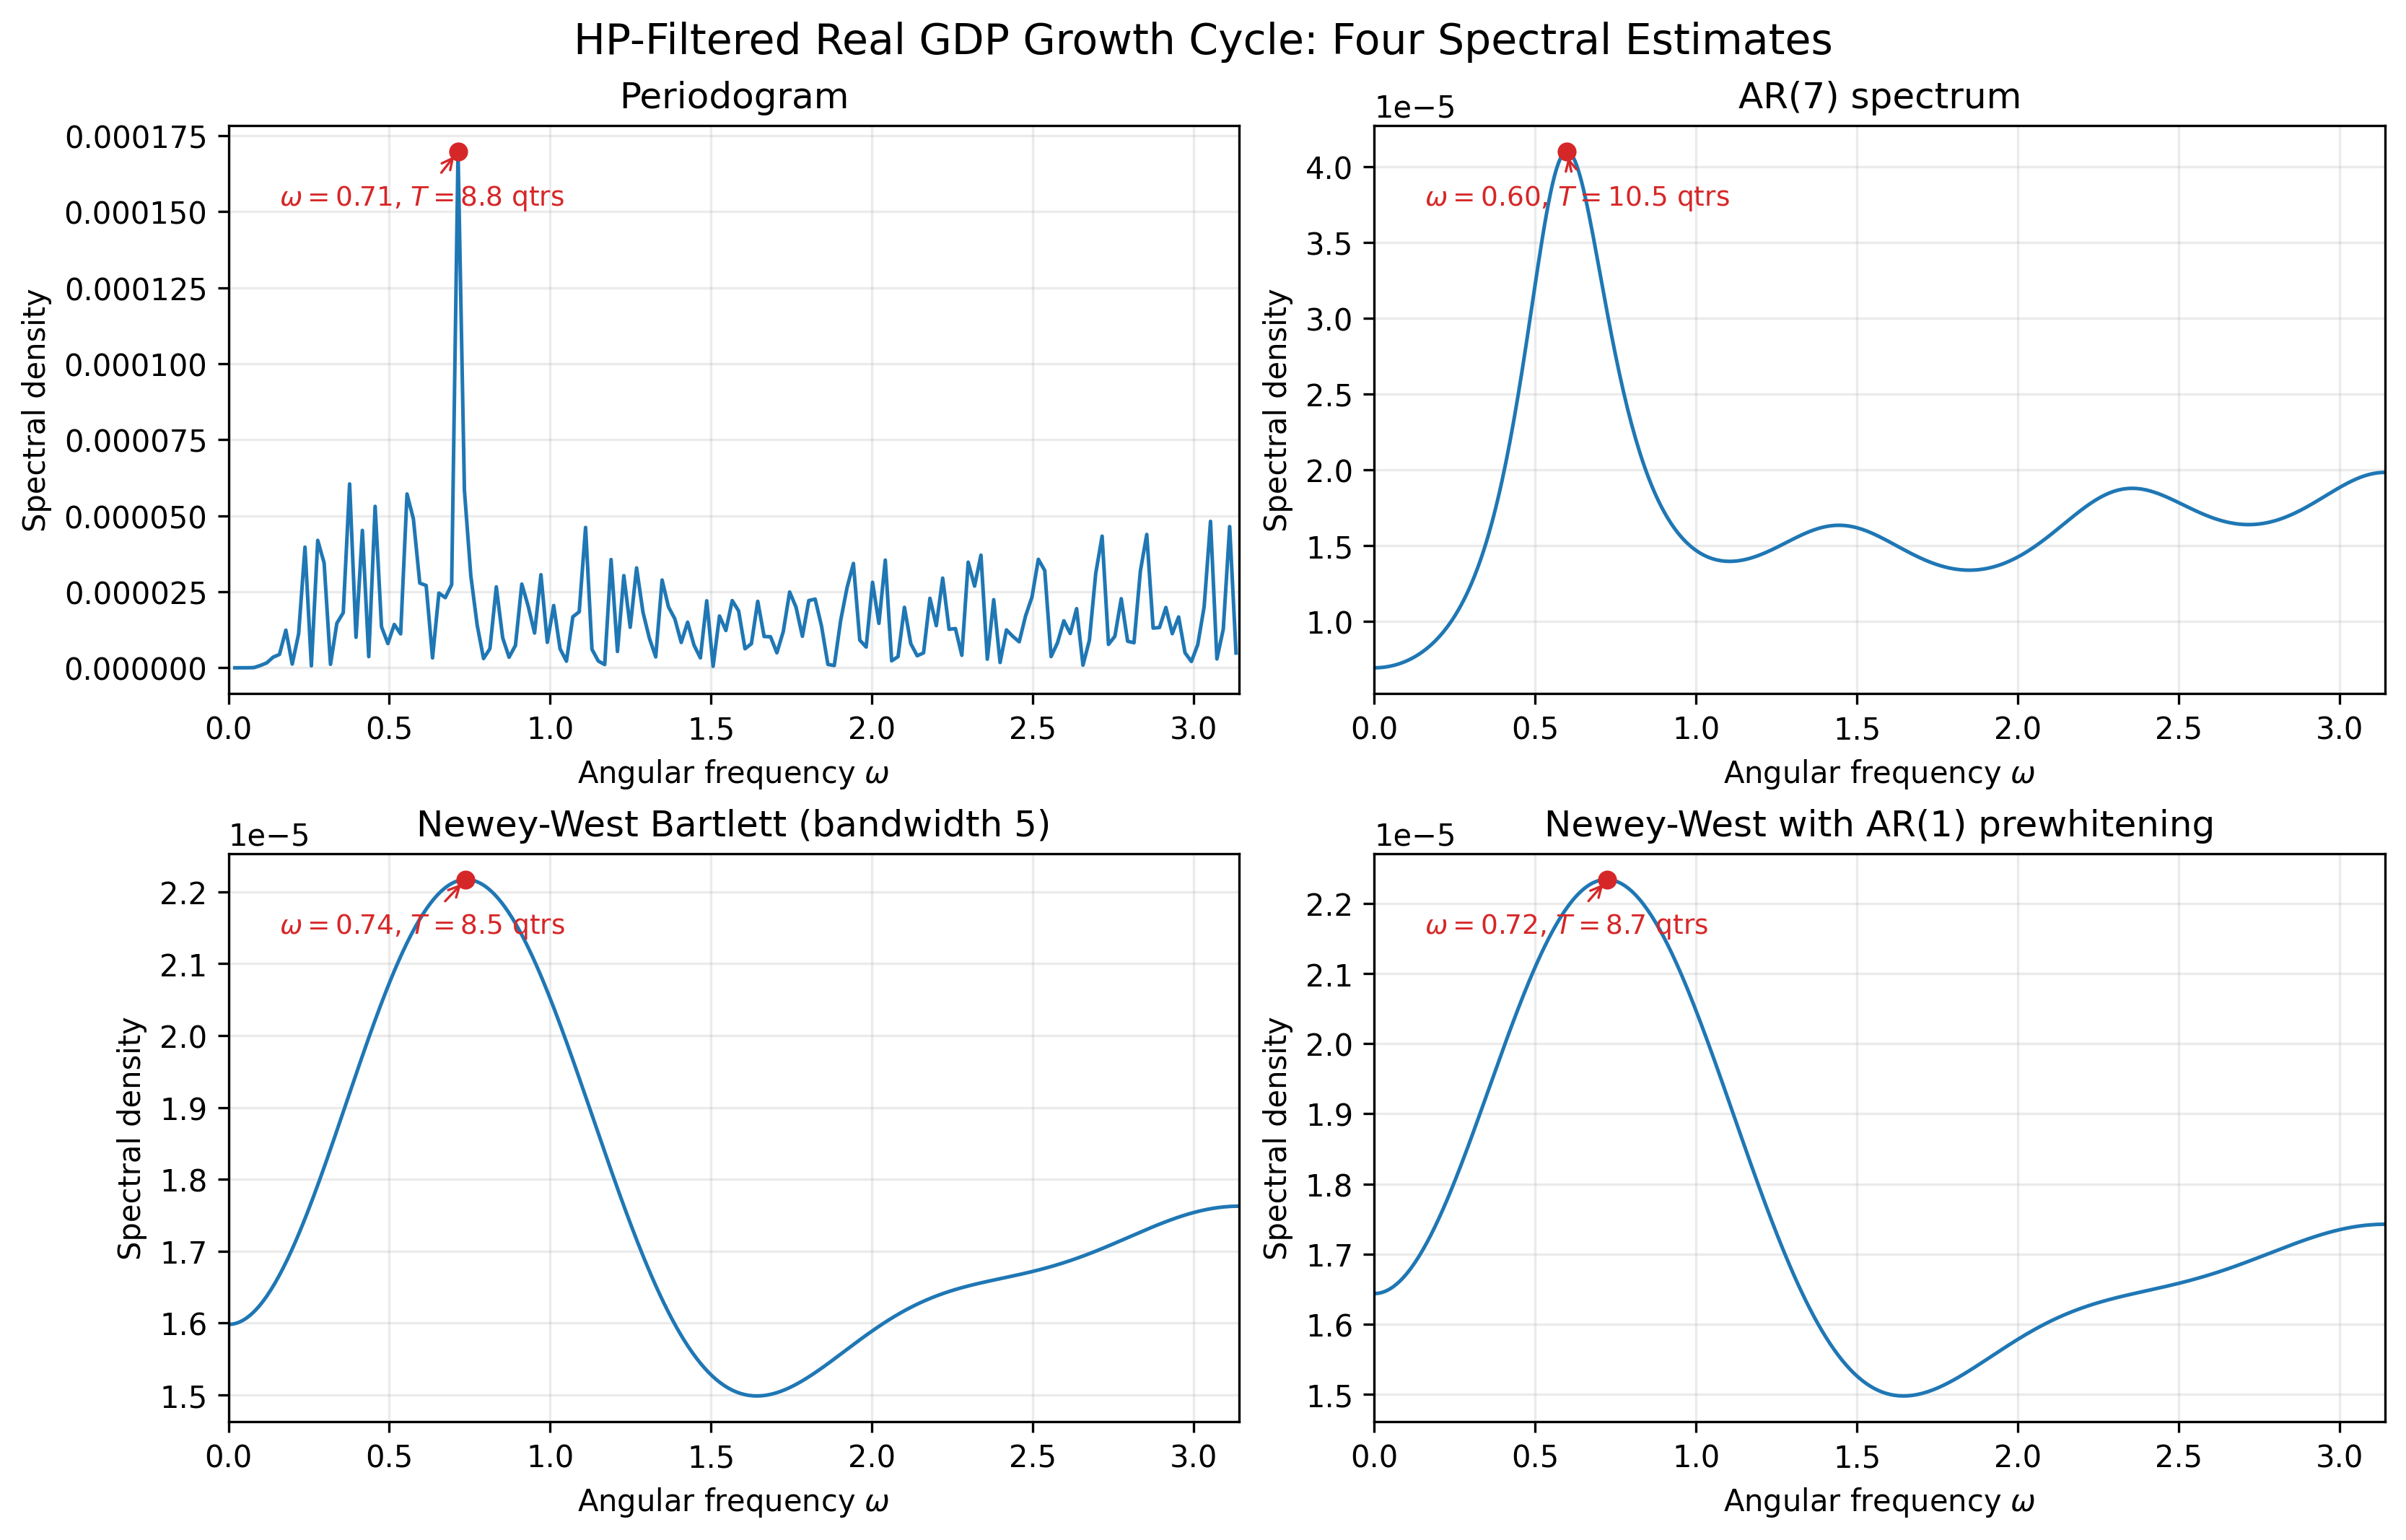
\includegraphics[width=0.9\textwidth]{rgdp_growth_four_spectra.png}
    \caption{Four spectral estimates for the HP-filtered real GDP growth cycle.}
    \label{fig:rgdp-growth-four-spectra}
\end{figure}

\begin{figure}[H]
    \centering
    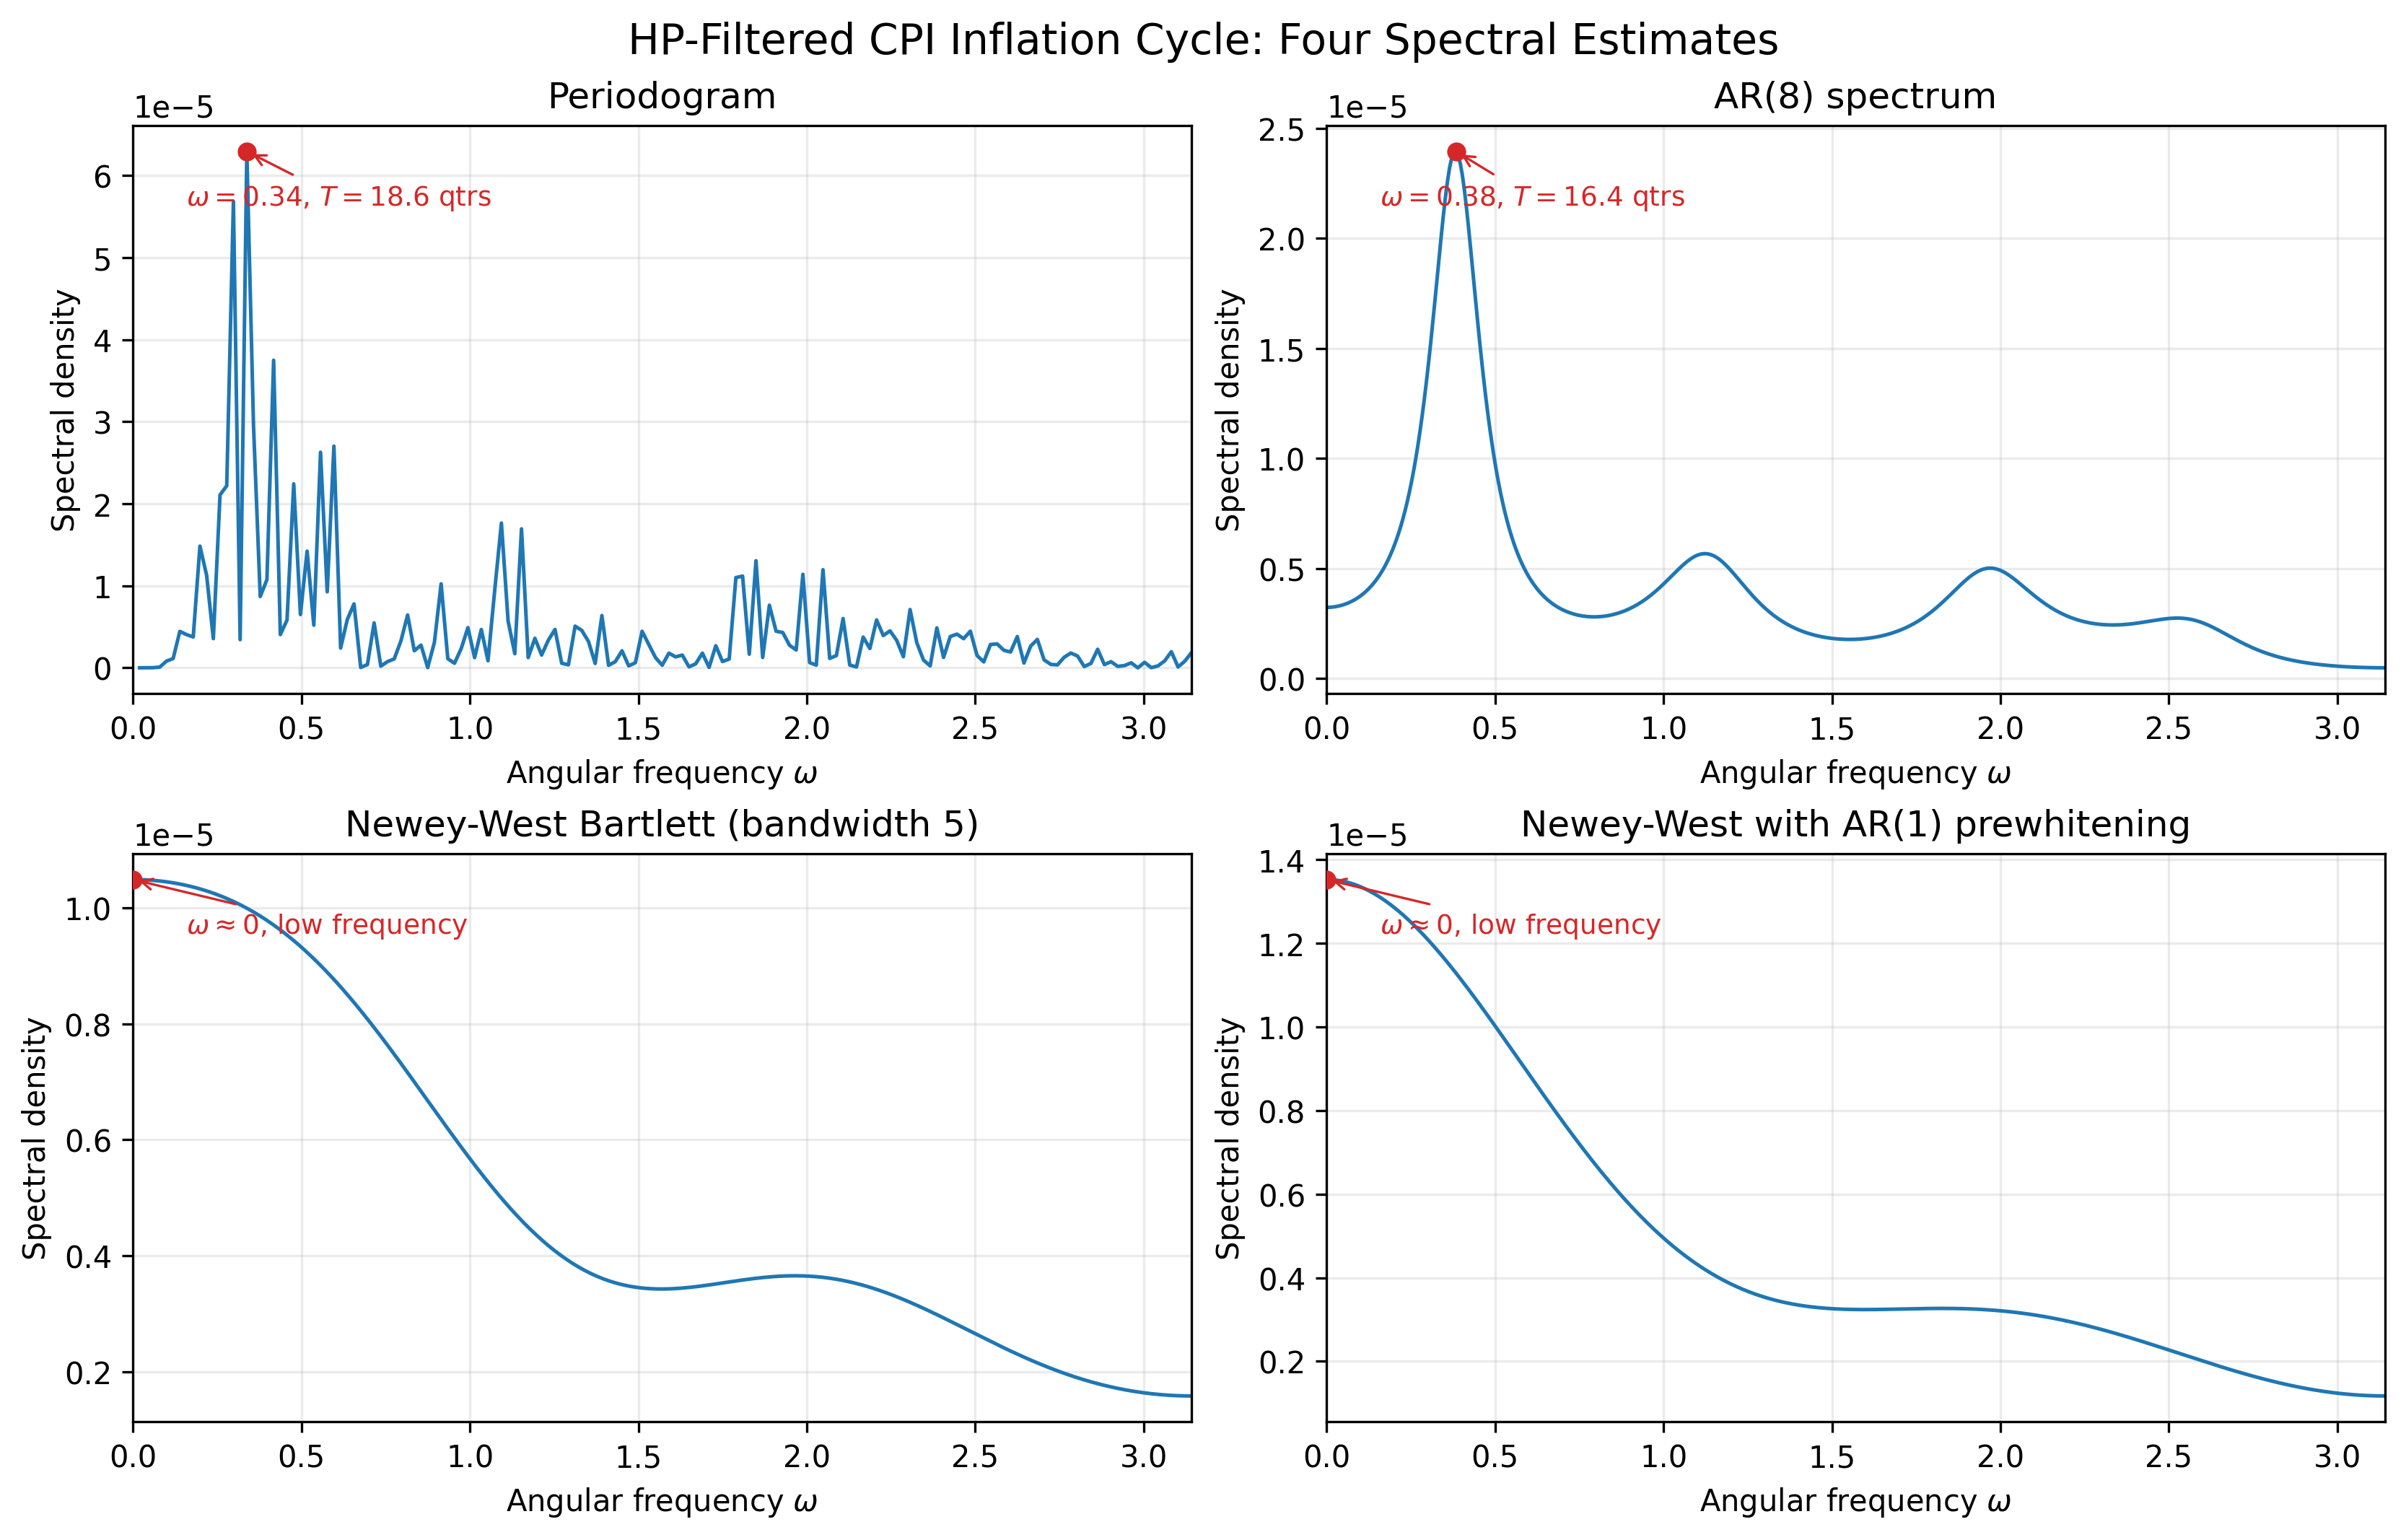
\includegraphics[width=0.9\textwidth]{cpi_inflation_four_spectra.png}
    \caption{Four spectral estimates for the HP-filtered CPI inflation cycle.}
    \label{fig:cpi-inflation-four-spectra}
\end{figure}



\end{document}